\section{Evaluation}
\label{sec:experiment}

%In this section, we perform extensive experiments on time series forecasting task of real-world datasets. %\peter{Do we still need toy experiments on synthetic data?}

We conducted extensive experiments with 9 methods (including our new methods) on 4 benchmark datasets for time series forecasting tasks.

\subsection{Methods for Comparison}
\label{sec:baseline}
%The following state-of-the-art methods are considered as comparisons for time series forecasting task. 
The methods in our comparative evaluation are the follows.
\begin{itemize}
    \item \AR stands for the autoregressive model, which is equivalent to the one dimensional VAR model. 
    \item \LRidge is the vector autoregression (VAR) model with L2-regularization
    %, which has been most popular for multivariate time series forecasting.
    \item \LSVR is the vector autoregression (VAR) model with Support Vector Regression loss \cite{vapnik1997support} . 
    %\item \TRMF is the autoregressive model using temporal regularized matrix factorization by \cite{Yu_NIPS_16}.
    \item \GP is the Gaussian Process for time series modeling. \cite{frigola2015bayesian,roberts2013gaussian}
    \item \VARMLP combines Multilayer Perception (MLP) and autoregressive model \cite{zhang2003time}. 
    \item \RNN is the Recurrent Neural Network model using GRU cell. %\peter{TODO}
    \item LST-L1 is our proposed LSTNet model with the absolute loss objective function.
    \item LST-L2 is our proposed LSTNet model with the square loss objective function.
\end{itemize}
For the single output methods above such as \AR, \LRidge, \LSVR and \GP, we just trained $n$ models independently, i.e., one model for each of the $n$ output variables.

\subsection{Metrics}
\label{sec:metrics} 
We consider three evaluation metrics defined as:
\begin{itemize}
	\item Root Relative Squared Error (RSE):
        \begin{equation*}
        RSE = \frac{\sqrt{\sum_{(i,t) \in \Omega_{Test}}(Y_{it} - \hat{Y}_{it})^2}}
        			{\sqrt{\sum_{(i,t) \in \Omega_{Test}} (Y_{it} - \mu(\bY))^2}}
        \end{equation*}
	%\item Relative Absolute Error (RAE) 
  %      \begin{equation*}
  %      RAE = \frac{\sum_{(i,t) \in \Omega_{Test}} |Y_{it} - \hat{Y}_{it}|}
  %      			{\sum_{(i,t) \in \Omega_{Test}} |Y_{it} - \mu(\bY)|}
  %      \label{eq:RAE}
  %      \end{equation*}   
  \item Empirical Correlation Coefficient (CORR)
      \begin{equation*}
      CORR =\frac{1}{n} \sum_{i=1}^n 
        \frac{\sum_t \big(Y_{it} - \mu({\bY}_i)\big) \big(\hat{Y}_{it} - \mu(\hat{\bY}_i)\big)}
      	     {\sqrt{\sum_t \big(Y_{it} - \mu({\bY}_i)\big)^2 \big(\hat{Y}_{it} - \mu(\hat{\bY}_i)\big)^2}}
      \label{eq:Correlation}
      \end{equation*}    
\end{itemize}
where $\mu(\cdot)$ is the mean function and $\bY,\hat{\bY} \in \mathbb{R}^{n\times T}$ are ground true signals and system prediction signals, respectively. RSE, the scaled version of Root Mean Square Error(RMSE), is designed as more interpretable evaluations across different datasets. RSE is lower value the better, while CORR higher value the better.

\subsection{Data}
\label{sec:data}
%We take a broad range of real-world data into consideration while examining the effectiveness of our proposed framework. 
We used four benchmark datasets which are publicly available. We denote time length $T$, number of variables $D$, and 
frequency between two samples $F$.
%Table \ref{tb:data-stats} summarizes the corpus statistics.
\begin{itemize}
    \item \traffic \footnote{\url{http://pems.dot.ca.gov}}: A collection of 48 months (2015-2016) hourly data from the California Department of Transportation. The data describes the road occupancy rates (between 0 and 1) measured by different sensors on San Francisco Bay area freeways. $T=17544$, $D=682$, $F$ is 1 hour. 
    %\item \wind \footnote{\url{https://www.kaggle.com/c/GEF2012-wind-forecasting}}: The wind power generation for $n=7$ wind power farm, measured in every hour. This dataset is from the Wind Forecasting track of Global Energy Forecasting Competition 2012. The data is available for period ranging from the 1st hour of 2009/7/1 to the 12th hour of 2012/6/28.
	%\item \temp \footnote{\url{https://www.ncdc.noaa.gov/crn/qcdatasets.html}}: The Temperature dataset is downloaded from NOAA website, which contains hourly temperature records for 146 major cities in the U.S.A from 2014 to 2016.
    \item \solar \footnote{\url{http://www.nrel.gov/grid/solar-power-data.html}} : the solar power production records in the year of 2006, which is sampled every 10 minutes from 137 PV plants in Alabama State. $T=52560$, $D=137$, $F$ is 10 minutes.
	\item \electricity \footnote{\url{https://archive.ics.uci.edu/ml/datasets/ElectricityLoadDiagrams20112014}}: The electricity consumption in kWh was recorded every 15 minutes from 2012 to 2014, for $n=321$ clients. We converted the data to reflect hourly consumption. $T=26304$, $D=321$, $F$ is 1 hour.
    \item \exchange: the collection of the daily exchange rates of eight foreign countries including Australia, British, Canada, Switzerland, China, Japan, New Zealand and Singapore ranging from 1990 to 2016. $T=7588$, $D=8$, $F$ is 1 day.
\end{itemize}

\iffalse
\begin{table}
	\begin{center}
        \resizebox{0.75\columnwidth}{!}{%
		\begin{tabular}{lrrrrrrrr} 
		\toprule
		Datasets 		 & $T$		 & $D$	& $L$		 \\
		\midrule
		\traffic 		 & 17,544  & 862 	& 1 hour	\\
    \solar			 & 52,560	 & 137	& 10 minutes\\
		\electricity & 26,304  & 321 	& 1 hour	\\
    \exchange		 & 7,588	 & 8		& 1 day		\\
    \bottomrule
		\end{tabular}
        }
        %\vspace{-0.125cm}
        \caption{Dataset Statistics, where $T$ is length of time series, $D$ is number of variables, $L$ is the sample rate.}
		\label{tb:data-stats}
	\end{center}
\end{table}
\fi

All datasets are split into training (60\%), validation (20\%) and test (20\%) set in chronological order. To facilitate future research in multivariate time series forecasting, we publicize all raw datasets and the one after preprocessing in the website
\footnote{\url{https://github.com/laiguokun/multivariate-time-series-data}}.

To examine the existence of long-term and/or short-term repetitive patterns in time series data, we plot autocorrelation graph for some randomly selected variables from the four datasets in Figure \ref{fig:autocorrelation}.
Autocorrelation is the correlation of a signal with a delayed copy of itself as a function of delay, defined as
	$R(\tau) =  \mathbb{E}[(X_t - \mu)(X_{t+\tau} - \mu)] / \sigma^2$
where $X_t$ is the time series signals, $\mu$ is mean and $\sigma^2$ is variance.
%In practice, we consider the empirical unbiased estimator to calculate the autocorrelation.  

In Figure \ref{fig:autocorrelation}, there are repetitive patterns with high autocorrelation in the \traffic, \solar and \electricity datasets, but not in the \exchange dataset. Furthermore, we observe a short-term daily pattern (in every 24 hours) and long-term weekly pattern (in every 7 days) in the \traffic and \electricity dataset, reflecting the expected regularity in highway traffics and electricity consumptions.  On the other hand, we hardly see any repetitive long-term patterns in the \exchange dataset, expect some short-term local continuity. 
These observations suggest for methods capable of leveraging both short-term and long-term repetitive patterns should outperforms on \electricity, \traffic and \solar dataset. In contrast, if the dataset does not contain such patterns (like in \exchange), the advantageous power of those methods may not lead a better performance.
%This key observation is later justified for the reason why our proposed models does not outperform other baseline models on this \exchange dataset.
%In the discussion of sec.\ref{sec:mixture}, the experiment result demonstrates the ability of LSTNet structure to model the complex mixture patterns.  

\begin{figure}[!ht]
\begin{subfigure}{.23\textwidth}
  \centering
  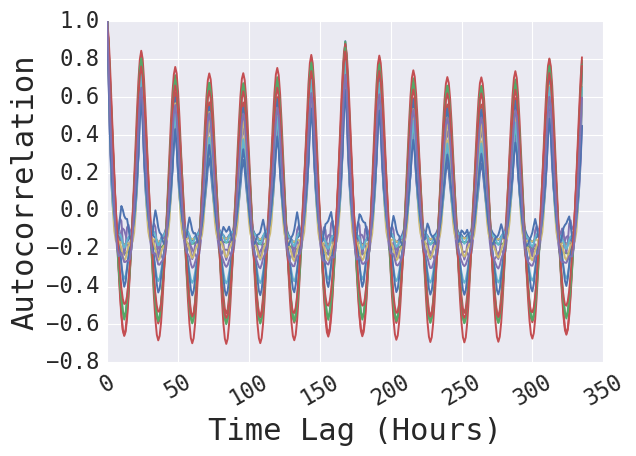
\includegraphics[width=\linewidth]{fig-auto/autocorr_traffic.png}
  \caption{\traffic dataset}
\end{subfigure}
\begin{subfigure}{.23\textwidth}
  \centering
  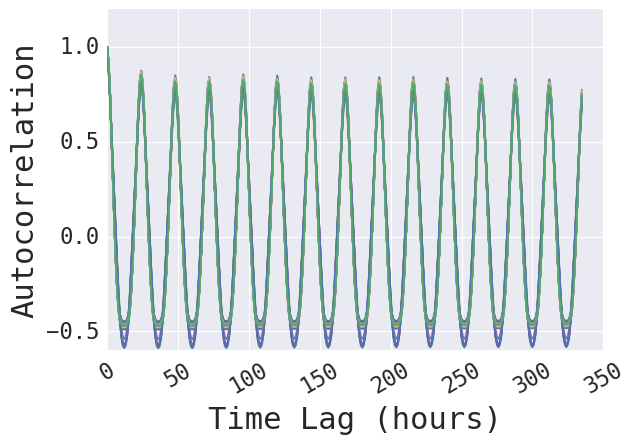
\includegraphics[width=\linewidth]{fig-auto/autocorr_solar.png}
  \caption{\solar dataset}
\end{subfigure}
\begin{subfigure}{.23\textwidth}
  \centering
  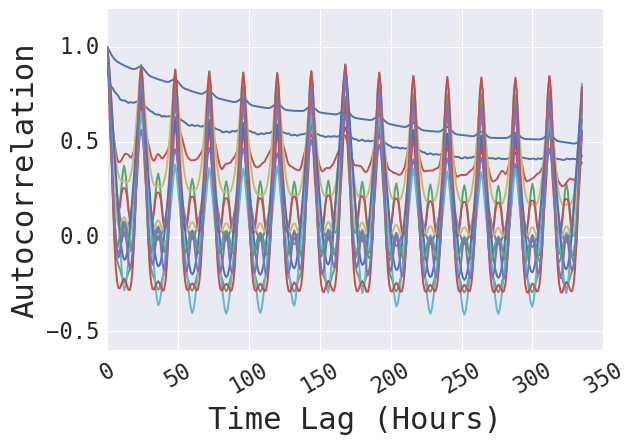
\includegraphics[width=\linewidth]{fig-auto/autocorr_electricity.png}
  \caption{\electricity dataset}
\end{subfigure}
\begin{subfigure}{.23\textwidth}
  \centering
  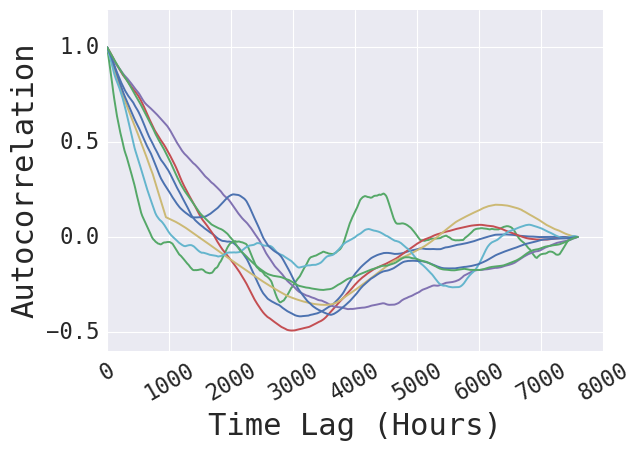
\includegraphics[width=\linewidth]{fig-auto/autocorr_exchange.png}
  \caption{\exchange dataset}
\end{subfigure}
%\vspace{-0.3cm}
\caption{Autocorrelation graphs of some sampled variables.}
\label{fig:autocorrelation}
%\vspace{-0.5cm}
\end{figure}
%\yiming{Peter or Guokun: Make the axis readable!}


\begin{table*}[!ht]
\centering
\resizebox{\textwidth}{!}{
\begin{tabular}{ll|cccc|cccc|cccc|cccc}
\toprule
Dataset &  
        & \multicolumn{4}{c|}{\solar}       & \multicolumn{4}{c|}{\traffic}
        & \multicolumn{4}{c|}{\electricity} & \multicolumn{4}{c}{\exchange}  \\
\midrule
				&
        & \multicolumn{4}{c|}{Horizon} & \multicolumn{4}{c|}{Horizon}
        & \multicolumn{4}{c|}{Horizon} & \multicolumn{4}{c}{Horizon} \\
\midrule
Methods 	& Metrics & 3 & 6 & 12 & 24 & 3 & 6 & 12 & 24 & 3 & 6 & 12 & 24 & 3 & 6 & 12 & 24 \\
\midrule
\multirow{1}{*}{\AR}
  & RSE 
  & 0.2435 & 0.3790 & 0.5911 & 0.8699 
  & 0.5991 & 0.6218 & 0.6252 & 0.6293
  & 0.0995 & 0.1035 & 0.1050 & 0.1054 
  & 0.0228 & 0.0279 & 0.0353 & 0.0445 \\	
  %& RAE 
  %& 0.1846 & 0.3242 & 0.5637 & 0.9221 
  %& 0.4491 & 0.4610 & 0.4700 & 0.4696
  %& 0.0579 & 0.0598 & 0.0603 & 0.0611 
  %& 0.0181 & 0.0224 & 0.0291 & 0.0378 \\
  \textbf{(0)} & CORR 
  & 0.9710 & 0.9263 & 0.8107 & 0.5314 
  & 0.7752 & 0.7568 & 0.7544 & 0.7519
  & 0.8845 & 0.8632 & 0.8591 & 0.8595 
  & 0.9734 & 0.9656 & 0.9526 & 0.9357 \\   
\midrule
\multirow{1}{*}{\LRidge}
  & RSE 
  & 0.2019 & 0.2954 & 0.4832 & 0.7287 
  & 0.5833 & 0.5920 & 0.6148 & 0.6025
  & 0.1467 & 0.1419 & 0.2129 & 0.1280 
  & 0.0184 & 0.0274 & 0.0419 & 0.0675\\
	%& RAE 
  %& 0.1227 & 0.2098 & 0.4070 & 0.6977 
  %& 0.4965 & 0.5115 & 0.5198 & 0.4846
  %& 0.0900 & 0.0933 & 0.1268 & 0.0779 
  %& 0.0144 & 0.0225 & 0.0358 & 0.0602\\
  \textbf{(0)} & CORR 
  & 0.9807 & 0.9568 & 0.8765 & 0.6803 
  & 0.8038 & 0.8051 & 0.7879 & 0.7862
  & 0.8890 & 0.8594 & 0.8003 & 0.8806 
  & 0.9784 & 0.9702 & 0.9543 & 0.9305 \\   
\midrule
\multirow{1}{*}{LSVR}
  & RSE 
	& 0.2021 & 0.2999 & 0.4846 & 0.7300 
  & 0.5740 & 0.6580 & 0.7714 & 0.5909
  & 0.1523 & 0.1372 & 0.1333 & 0.1180 
  & 0.0189 & 0.0284 & 0.0425 & 0.0662 \\
	%& RAE  
  %& 0.1082 & 0.2451 & 0.4362 & 0.6180 
  %& 0.4629 & 0.5483 & 0.7454 & 0.4761
  %& 0.0858 & 0.0816 & 0.0762 & 0.0690
  %& 0.0148 & 0.0231 & 0.0360 & 0.0576 \\
  \textbf{(0)} & CORR 
  & 0.9807 & 0.9562 & 0.8764 & 0.6789 
  & 0.7993 & 0.7267 & 0.6711 & 0.7850 
  & 0.8888 & 0.8861 & 0.8961 & 0.8891 
  & 0.9782 & 0.9697 & 0.9546 & 0.9370 \\   
%\midrule
%\multirow{1}{*}{TRMF}
%  & RSE 
%  & 0.2473 & 0.3470 & 0.5597 & 0.9005 
%  & 0.6708 & 0.6261 & 0.5956 & 0.6442
%  & 0.1802 & 0.2039 & 0.2186 & 0.3656 
%  & 0.0351 & 0.0875 & 0.0494 & 0.0563 \\
%	%& RAE 
%  %& 0.1481 & 0.2165 & 0.3717 & 0.6526
%  %& 0.5887 & 0.5295 & 0.4479 & 0.5256 
%  %& 0.1064 & 0.1175 & 0.1571 & 0.2686 
%  %& 0.0302 & 0.0654 & 0.0464 & 0.0510\\
%  \textbf{(0)} & CORR 
%  & 0.9703 & 0.9418 & 0.8475 & 0.5598
%  & 0.6964 & 0.7430 & 0.7748 & 0.7278 
%  & 0.8538 & 0.8424 & 0.8304 & 0.7471 
%  & 0.9142 & 0.8123 & 0.8993 & 0.8678 \\
\midrule
\multirow{1}{*}{GP}
  & RSE 
	& 0.2259 & 0.3286 & 0.5200 & 0.7973
  & 0.6082 & 0.6772 & 0.6406 & 0.5995
  & 0.1500 & 0.1907 & 0.1621 & 0.1273 
  & 0.0239 & 0.0272 & 0.0394 & 0.0580 \\
	%& RAE 
  %& 0.1419 & 0.2189 & 0.4095 & 0.7599
  %& 0.5148 & 0.5759 & 0.5316 & 0.4829
  %& 0.0907 & 0.1137 & 0.1043 & 0.0776
  %& 0.0230 & 0.0239 & 0.0355 & 0.0547 \\
  \textbf{(0)} & CORR 
  & 0.9751 & 0.9448 & 0.8518 & 0.5971
  & 0.7831 & 0.7406 & 0.7671 & 0.7909
  & 0.8670 & 0.8334 & 0.8394 & 0.8818
  & 0.8713 & 0.8193 & 0.8484 & 0.8278\\
\midrule
\multirow{1}{*}{VARMLP}
  & RSE 
	& 0.1922 & 0.2679 & 0.4244 & 0.6841 
  & 0.5582 & 0.6579 & 0.6023 & 0.6146 
  & 0.1393 & 0.1620 & 0.1557 & 0.1274
  & 0.0265 & 0.0304 & 0.0407 & 0.0578\\
  %& RAE  
  %& 0.1051 & 0.1635 & 0.3102 & 0.6084 
  %& 0.4510 & 0.5434 & 0.4947 & 0.5474
  %& 0.0970 & 0.1171 & 0.1261 & 0.0883
  %& 0.0244 & 0.0268 & 0.0356 & 0.0520 \\
  \textbf{(0)} & CORR 
  & 0.9829 & 0.9655 & 0.9058 & 0.7149 
  & 0.8245 & 0.7695 & 0.7929 & 0.7891
  & 0.8708 & 0.8389 & 0.8192 & 0.8679
  & 0.8609 & 0.8725 & 0.8280 & 0.7675 \\
\midrule
\multirow{1}{*}{RNN-GRU}
  & RSE 
  & 0.1932 & 0.2628 & 0.4163 & 0.4852 
  & 0.5358 & 0.5522 & 0.5562 & 0.5633 
  & 0.1102 & 0.1144 & 0.1183 & 0.1295 
  & 0.0192 & 0.0264 & 0.0408 & 0.0626\\
  %& RAE 
  %& 0.0986 & 0.1389 & 0.2226 & 0.2822 
  %& 0.3596 & 0.3747 & 0.3890 & 0.3965
  %& 0.0765 & 0.0806 & 0.0836 & 0.0829 
  %& 0.0157 & 0.0224 & 0.0372 & 0.0572\\
  \textbf{(0)} & CORR 
  & 0.9823 & 0.9675 & 0.9150 & 0.9823
  & 0.8511 & 0.8405 & 0.8345 & 0.8300
  & 0.8597 & 0.8625 & 0.8472 & 0.8651 
  & 0.9786 & 0.9712 & 0.9531 & 0.9223\\
\midrule
\multirow{}{*}{LSTNet-Skip}
  & RSE 
  & 0.1843 & 0.2559 & 0.3254 & 0.4636 
  & 0.4849 & 0.4995 & 0.5110 & 0.5221 
  & 0.0864 & 0.0931 & 0.1007 & 0.1060 
  & 0.0232 & 0.0302 & 0.0382 & 0.0570\\
  %& RAE 
  %& 0.0923 & 0.1360 & 0.1894 & 0.3484 
  %& 0.3163 & 0.3307 & 0.3443 & 0.3509
  %& 0.0519 & 0.0563 & 0.0572 & 0.0571 
  %& 0.0189 & 0.0253 & 0.0313 & 0.0498\\
  \textbf{(0)} & CORR 
  & 0.9843 & 0.9690 & 0.9467 & 0.8870
  & 0.8721 & 0.8645 & 0.8576 & 0.8552
  & 0.9283 & 0.9135 & 0.9077 & 0.9119 
  & 0.9746 & 0.9670 & 0.9517 & 0.9314\\
%\midrule                                                
%\multirow{2}{*}{LST-L2}
%  & RSE 
%	& 0.1988 & 0.2726 & 0.3780 & 0.4928
%	& \textbf{0.4777} & \textbf{0.4893} & \textbf{0.4950} & \textbf{0.4973}
%  & 0.0967 & 0.1013 & 0.1017 & 0.1010
%	& 0.0226 & 0.0280 & 0.0356 & 0.0449\\
%	& RAE 
%	& 0.1126 & 0.1796 & 0.2593 & 0.3124
%	& 0.3541 & 0.3830 & \textbf{0.3749} & \textbf{0.3887}
%  & 0.0581 & 0.0598 & 0.0601 & 0.0600
%	& 0.0180 & 0.0226 & 0.0296 & 0.0378\\
%  \textbf{(10)} & CORR 
%  & 0.9826 & 0.9639 & 0.9255 & 0.8670 
%  & \textbf{0.8715} & \textbf{0.8627} & \textbf{0.8614} & \textbf{0.8588}
%  & 0.8941 & 0.8764 & 0.8765 & 0.8848
%  & 0.9735 & 0.9658 & 0.9511 & 0.9354\\ 
                                                
\bottomrule
\end{tabular}
}
\caption{Results summary: 1) bold face indicates the best result of each column in a particular metric; and 2) the total number of bold-faced results of each method is listed under the method name within parentheses. }
\label{tb:result}
%\vspace{-0.5cm}
\end{table*}




\subsection{Experimental Details}
%\peter{TODO:modify description of window size and add GP, TRMF}
We conduct grid search over all tunable hyper-parameters on the validation set for each method and dataset. Specifically, all methods share the same grid search range of the window size $q$ ranging from $\{2^0,2^1,\ldots,2^9\}$ if applied. For \LRidge and \LSVR, the regularization coefficient $\lambda$ is chosen from $\{2^{-10}, 2^{-8}, \ldots, 2^{8}, 2^{10}\}$. For \GP, the RBF kernel bandwidth $\sigma$ and the noise level $\alpha$ are chosen from $\{2^{-10}, 2^{-8}, \ldots, 2^{8}, 2^{10}\}$. For \TRMF, the hidden dimension is chosen from $\{2^2, \ldots, 2^6\}$ and the regularization coefficient $\lambda$ is chosen from $\{0.1, 1, 10\}$.  For LSTNet, we adopted the hidden dimension of the Recurrent and Convolutional layer is chosen from $\{50,100,200\}$, and $\{20,50,100\}$ for Recurrent-skip layer. The skip-length $p$ of Recurrent-skip layer is set as 24 for the \traffic and \electricity dataset, and tuned range from $2^1$ to $2^6$ for the \solar and \exchange datasets. The regularization coefficient of the AR component is chosen from $\{0.1,1,10\}$ to achieve the best performance. The Adam\cite{kingma2014adam} algorithm is utilized to optimize the parameters of our model.


\subsection{Main Results}
\label{sec:result}

%Following the problem format in Sec.\ref{sec:format}, we perform the time series forecasting with $horizon = \{3,6,12,24\}$ across all datasets. The horizons are chosen by considering the real demanding of different applications. First, for traffic usage and electricity consumption, people are more care about the situation in next several hours to a day. In the energy output of solar farms, the prediction dozens of minutes ahead are more valuable compared to the long horizon. Because, researchers usually leverage satellite cloud pictures, which have a low refresh frequency, to forecast output in next half or a day. In the economic area, people only demand the prediction few seconds ahead, but the minimum granularity of public economic datasets is a day. However, it is still a good example of the time series signals without the repetitive patterns.   

Table \ref{tb:result} summarizes the evaluation results. We set $horizon = \{3,6,12,24\}$, which means the horizons was set from 3 to 24 hours for the forecasting over the \electricity and \traffic data, from 30 to 240 minutes over the \solar data, and from 3 to 24 days over the \exchange data. The larger the horizons, the harder the prediction tasks. The best result for each (data, metric) pair is highlighted in bold face in this table.  The total count of the bold-faced results is 28 for LST-L1 (one version of the proposed LSTNet), 10 for LST-L2 (the other version of our LSTNet), 5 for AR, 4 for LRidge, and between 0 to 2 for the rest of the methods.  

Clearly, LSTNet has the dominating performance on the first three datasets (\electricity, \solar and \traffic), especially in the settings with the large horizon. In the $horizon=24$ settings, LSTNet model improves the best state-of-the-art result by $35\%$ in \solar, $20\%$ in \traffic and $5\%$ in \electricity dataset in RSE evaluation metric. But it is slightly worse than AR and LRidge on the \exchange dataset. Why?  Recall that in Section \ref{sec:data} and Figure  \ref{fig:autocorrelation} we used the autocorrelation curves of these datasets to show the existence of  repetitive patterns in the \solar, \traffic and \electricity datasets but not in \exchange.  The current results provide empirical evidence for the success of LSTNet models in modeling long-term and short-term dependency patterns when they do occur in data.  Otherwise, LSTNet performed comparably  with the better ones (AR and LRidge) among the representative baselines.  The robustness of LSTNet is also due to its inclusion of the autoregressive model as a component, which we will discuss further in next section.


%show our proposed models outperform baseline algorithms in all evaluation metrics and in all settings of \electricity, \solar and \traffic datasets, except $horizon = 3$ of \solar data, which is slightly below the \VARMLP model. In the most difficult situation of each dataset, where $horizon = 12,24$, our models enhance the state-of-the-art results by 5\% to 30\%. The outstanding accuracy in long-horizon forecasting settings gives the evidence of the ability of the LSTNet to model the mixture of sophisticate patterns. However, in \exchange dataset,  because of lacking the dependencies in the time dimension, LSTNet structure cannot enhance the state-of-the-art result. But they are still at the same level.

Compared the results of univariate AR with that of the multivariate baseline methods, we see that in some datasets, i.e. \solar and \traffic, the multivariate is stronger, but weaker otherwise, which means that the richer input information would causes overfitting in the traditional multivariate approaches. In contrast, the LSTNet has robust performance in different situations, partly due to its  autoregressive component, which we will discuss further in Section \ref{sec:ablation}.

%In \electricity dataset, the performance of \LSVR model dominates the \LRidge model. It is the motivation that we try to leverage the L1-loss objective function in the LSTNet architecture. Across different datasets, the LST-L1 gains better result in \electricity and \solar datasets, and the LST-L2 is better in \traffic. So it is determined by the dataset that which one, L1 or L2, is the better objective function choice for our framework.




\subsection{Ablation Study}
\label{sec:ablation}
%To demonstrate the efficiency of our framework design, a careful ablation study is conducted. Specifically, we remove each component one at a time in our LSTNet framework to see which yields the largest performance decreases. First, we name the LSTNet without different components as follows.
To examine the importance of each component in our framework, we conducted a set of ablation tests.  We denote \textbf{LSTw/oskip}, \textbf{LSTw/oCNN}, \textbf{LSTw/oAR} as the LSTNet models without the Recurrent-skip, the Convolution, the AR component, respectively. 

%\begin{itemize}
%\item LSTw/oskip: The LSTNet models without the Recurrent-skip component.
%\item LSTw/oCNN: The LSTNet models without the Convolutional component.
%\item LSTw/oAR: The LSTNet models without the AR component.
%\end{itemize}

%Because the advantage of the L1 and L2 loss function is unstable across different datasets, the objective functions of LSTw/oskip, LSTw/oCNN and LSTw/oAR models for a dataset are determined by the performance of the LST-L1 and LST-L2 in that dataset. 
For different baselines, we tune the hidden dimension of models such that they have the similar numbers of model parameters to the LSTNet model, which eliminates the performance enhance introduced by the number of the model parameters.

%The ablation tests are conducted in the \electricity, \solar and \traffic datasets. 
The results are shown in Figure \ref{fig:ablation} \footnote{We omit the results on \traffic and \exchange dataset due to the space limits as it shows similar trends in Figure \ref{fig:ablation}}. We observe that removing the Skip and CNN components in (\textbf{LSTw/oCNN} or \textbf{LSTw/oskip}) caused certain performance drops. All the components of LSTNet together leads to the robust performance of our approach on all the datasets. Also note that removing the AR component (in LSTw/oAR) caused the most significant performance drops on \electricity, but not on \solar dataset.

%and they show the complete LSTNet structure is the best model. We can find that the advantage of complete LSTNet model becomes more obviously with the increasing of horizon, which mean harder settings in our assignment. And when horizon is small, we may directly utilized the recent data and continuous property of the time series data to make a pretty precise prediction. In another hand, with horizon increasing, the forecasting task requires us to leverage the long-term patterns and sophisticate dependencies between the variables better, and the LSTNet architecture is designed to tackle this challenge. 

%The ablation study of the \electricity dataset demonstrates the crucial role of AR component in the specific datasets. And from Table \ref{tb:result}, we can also see 
%vanilla Auto-regression is especially a strong baseline in this dataset.  The reason is same as what is argued in Section \ref{sec:AR}. 

The conclusion is that our architecture design is most robust across all experiment settings, especially with the large horizons.

\begin{figure}[!ht]
  \begin{subfigure}{.22\textwidth}
    \centering
    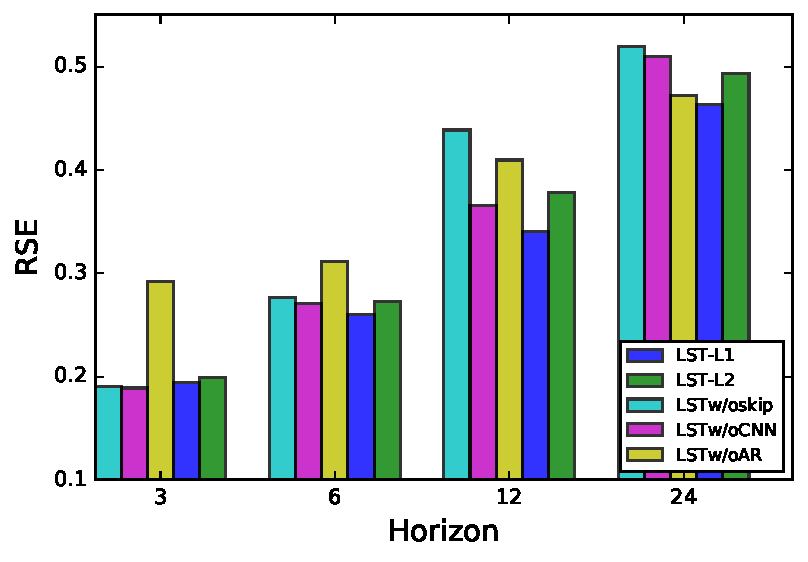
\includegraphics[width=\linewidth]{fig/rmse-solar.pdf}
    %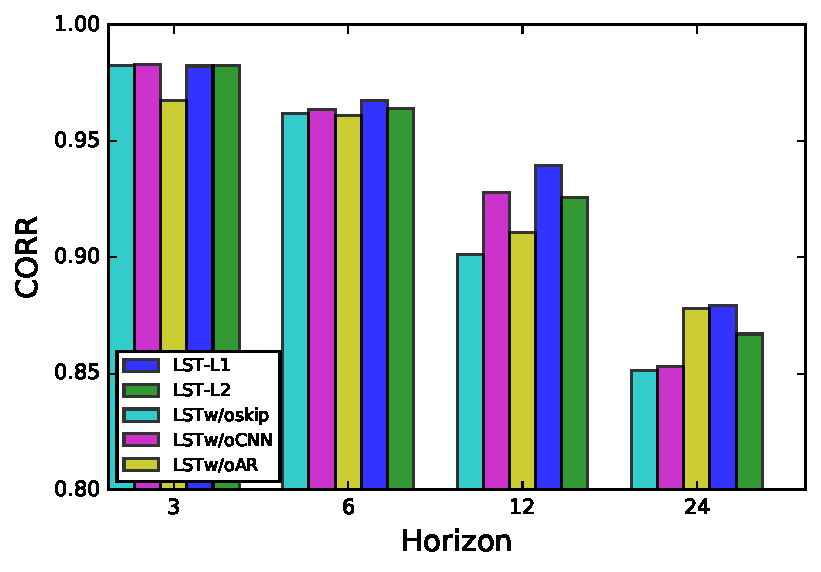
\includegraphics[width=.4\linewidth]{fig/corr-solar.pdf}
    %\vspace{-0.3 cm}
    \caption{\solar dataset}
  \end{subfigure}
  %\begin{subfigure}{.22\textwidth}
  %  \centering
  %  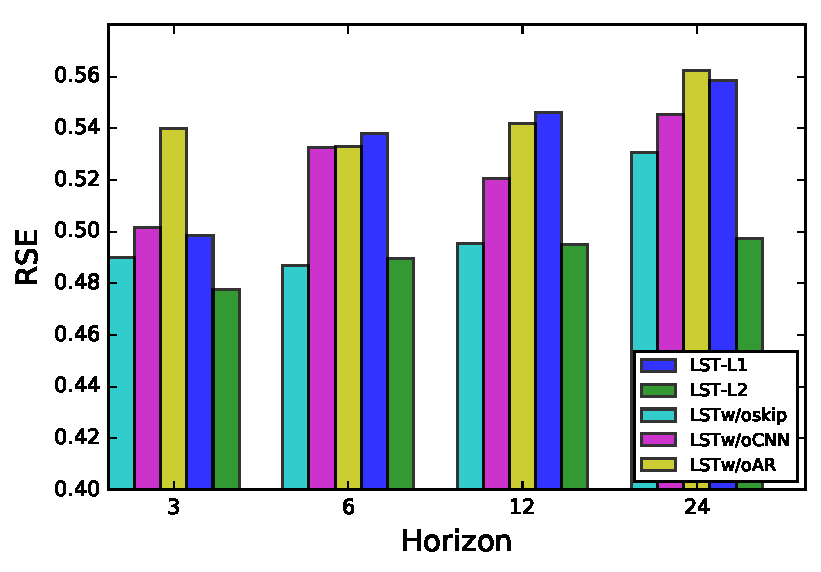
\includegraphics[width=\linewidth]{fig/rmse-traffic.pdf}
  %  %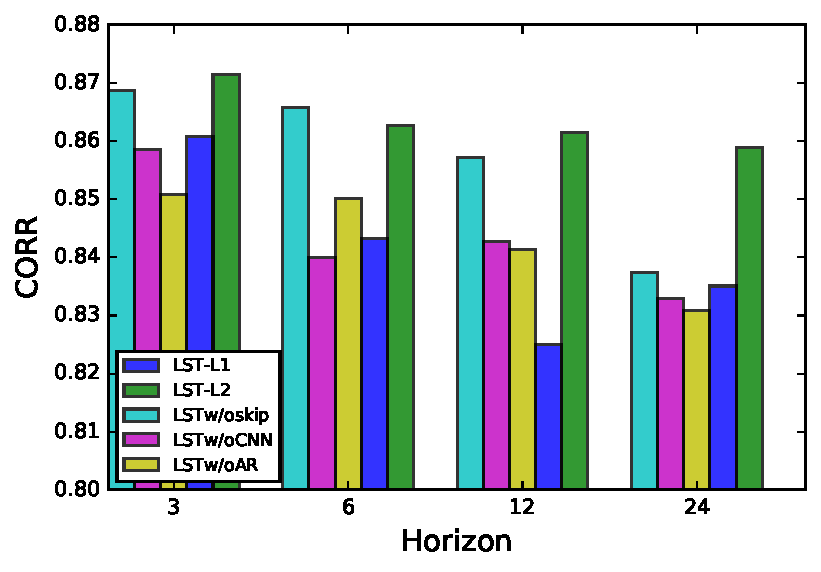
\includegraphics[width=.4\linewidth]{fig/corr-traffic.pdf}
  %  %\vspace{-0.3 cm}
  %  \caption{\traffic dataset}
  %\end{subfigure}
  \begin{subfigure}{.22\textwidth}
    \centering
    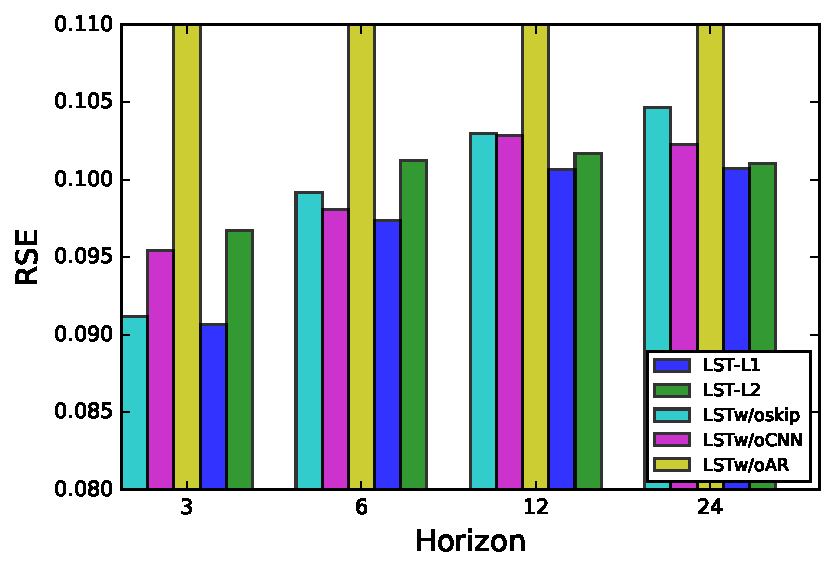
\includegraphics[width=\linewidth]{fig/rmse-ele.pdf}
    %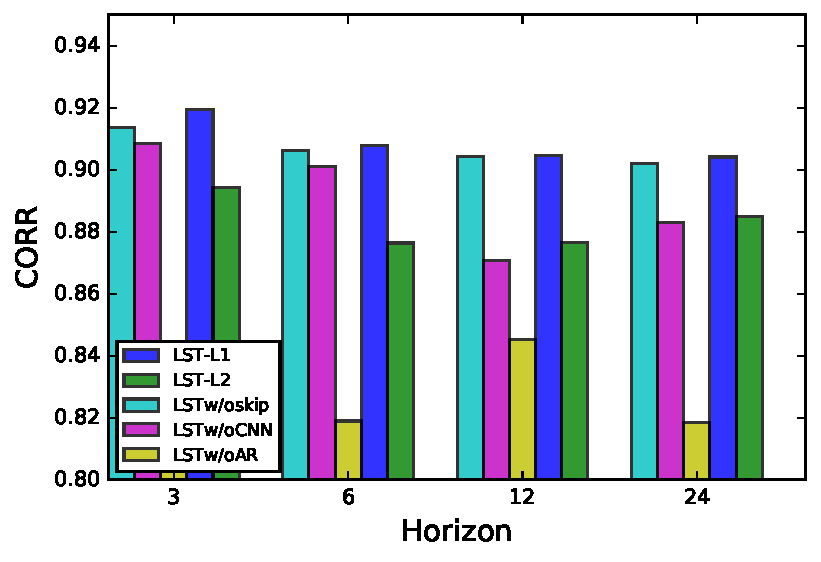
\includegraphics[width=.4\linewidth]{fig/corr-ele.pdf}
    %\vspace{-0.3cm}
    \caption{\electricity dataset}
  \end{subfigure}
  %\begin{subfigure}{.22\textwidth}
  %  \centering
  %  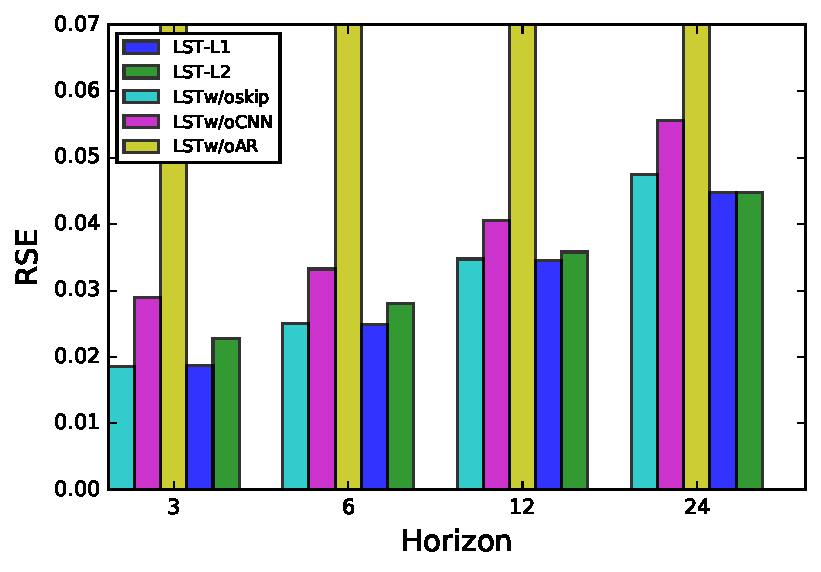
\includegraphics[width=\linewidth]{fig/rmse-exchange.pdf}
  %  %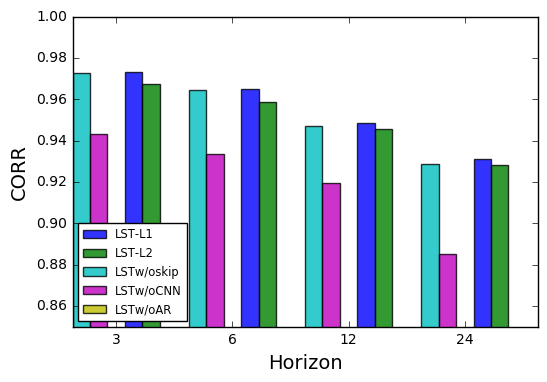
\includegraphics[width=.4\linewidth]{fig/corr-ex.png}
  %  %\vspace{-0.3 cm}
  %  \caption{\exchange dataset}
  %\end{subfigure}
  
  \caption{Results of LSTNet in the ablation tests.}
  \label{fig:ablation}
\end{figure}


\iffalse
As for why the AR component would have such an important role, our interpretation is that AR is generally robust to the sudden changes in data. To empirically validate this intuition we plot one dimension (one variable) of the time series signals in the electricity consumption dataset for the duration from 1 to 5000 hours in Figure \ref{fig:electricity}, where the blue curve is the true data and the red curve is the system-forecasted signals. We can see that the true consumption suddenly increases around the 1000th hour, and that LST-L1 successfully captures this sudden change but LSTw/oAR fails to react properly.  In other words, the neural-network component in LSTNet may not be sufficiently sensitive to random scale fluctuations in data (which is typical in \electricity data possibly due to random events for public holidays or temperature turbulence, etc.), while the simple linear AR model can make a proper adjustment in the forecasting.

\begin{figure}[!ht]
\begin{subfigure}{.23\textwidth}
  \centering
  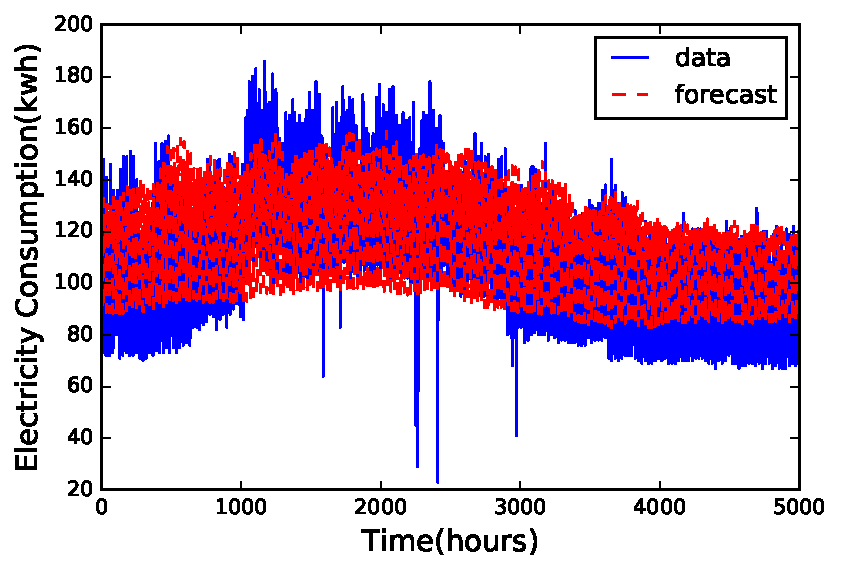
\includegraphics[width=\linewidth]{fig/woar.pdf}
  %\vspace{-0.5 cm}
  \caption{LSTNet w/o AR}
\end{subfigure}
\begin{subfigure}{.23\textwidth}
  \centering
  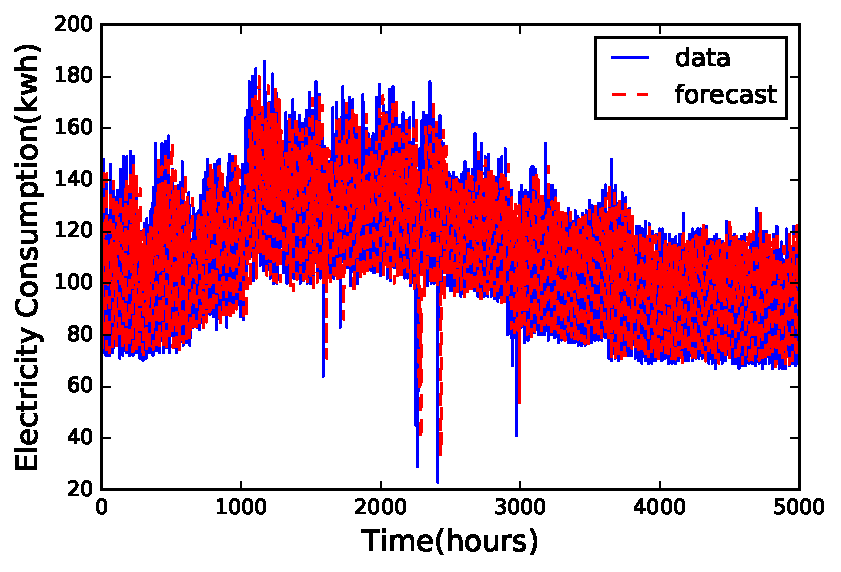
\includegraphics[width=\linewidth]{fig/war.pdf}
  %\vspace{-0.5 cm}
  \caption{LSTNet}
\end{subfigure}
\caption{The predicted time series (red) versus the true data (blue) on \electricity dataset with $horizon = 24$}
\label{fig:electricity}
%\vspace{1cm}
\end{figure}

%The LSTw/oAR fails to react very well to the fluctuated scale, and the prediction result is relatively conservative. In contrast, the complete LSTNet model can automatically adjust the prediction based on the input scale. What's more, this kind of random scale fluctuation is common in the \electricity data. One possible reason for this phenomenon is that the electricity consumption is frequently influenced by the factors hard to predict based on the history electricity consumption, e.g. the public holiday events and the temperature turbulence. However, the simple linear model adjusts the output scale according to the input by nature. After leveraging the AR component, the LSTNet structure is robust to this kind of data style. 

In summary, this ablation study clearly justifies the efficiency of our architecture design. All components have contributed to the excellent and robust performance of LSTNet.
\fi


\subsection{Mixture of long- and short-term patterns}
%\vspace{-0.1cm}
\label{sec:mixture}
To illustrate the success of LSTNet in modeling the mixture of short-term and long-term recurring patterns, Figure \ref{fig:traffic} compares the performance of LSTNet and VAR on an specific time series (one of the output variables) in the \traffic dataset. Note that the true signal (in blue) of traffic occupancy are very different on Fridays and Saturdays, and another on Sunday and Monday.

The figure shows that the VAR model is only capable to deal with the short-term patterns. The pattern of prediction results of the VAR model only depend on the day before the predictions. We can clearly see that the results of it in Saturday (2rd and 9th peaks) and Monday (4th and 11th peaks) is different from the ground truth, where the ground truth of Monday (weekday) has two peaks, one peak for Saturday (weekend). In the contrary, our proposed LSTNet model performs two patterns for weekdays and weekends respectfully. This example proves the ability of LSTNet model to memorize short-term and long-term recurring patterns simultaneously, which the traditional forecasting model is not equipped, and it is crucial in the prediction task of the real world time series signals. 
%However, the VAR model (part (a) of the figure) cannot learn such a distinction but predict the similar local patterns for both days instead. LSTNet, on the other hand (part (b) of the figure), successfully captures both the different repeating patterns on Mondays and Saturdays, and the local patterns within each day.




\begin{figure}[!ht]
  \begin{subfigure}{.23\textwidth}
    \centering
    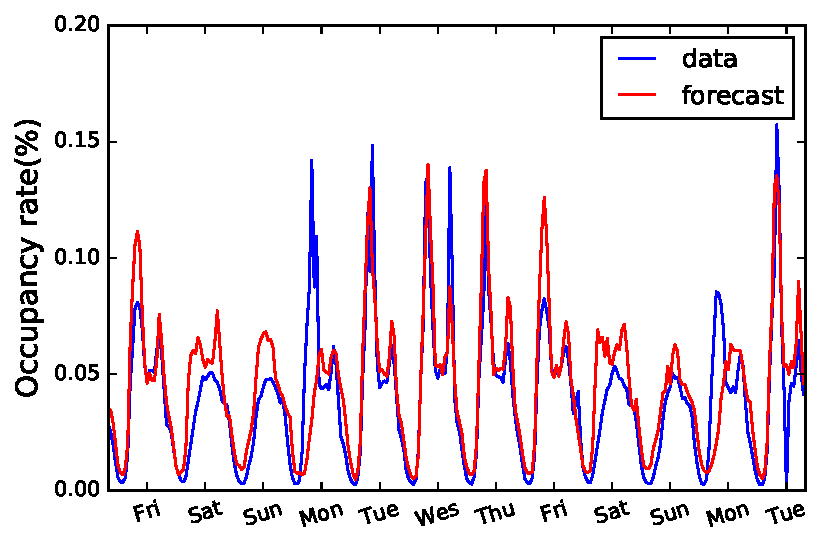
\includegraphics[width=\linewidth]{fig/traffic-var.pdf}
    \caption{VAR}
    \label{fig:tra-var}
  \end{subfigure}
  \begin{subfigure}{.23\textwidth}
    \centering
    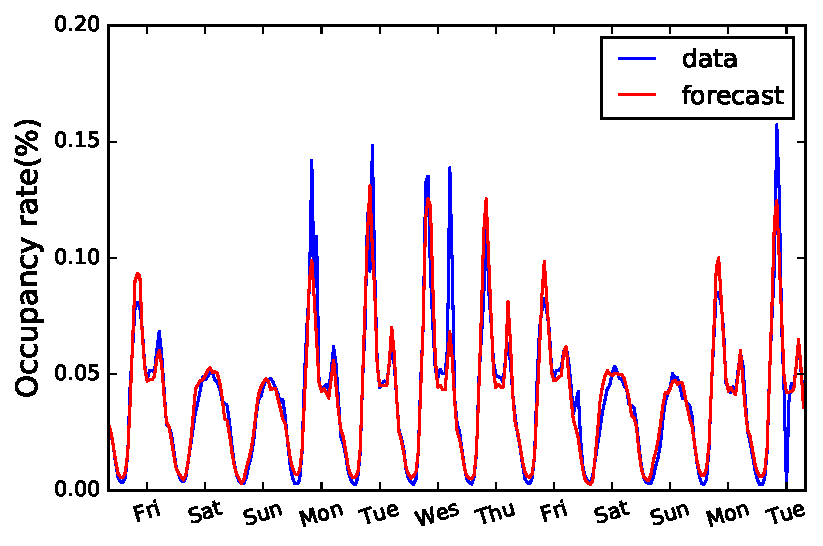
\includegraphics[width=\linewidth]{fig/traffic-tnn.pdf}
    \caption{LSTNet}
    \label{fig:tra-tnn}
  \end{subfigure}
  
  \caption{The true time series (blue) and the predicted ones (red) for one variable in the \traffic dataset. The x axis indicates the week days and the forecasting $horizon = 24$.}
  %\vspace{-0.5 cm}
  \label{fig:traffic}
\end{figure}



